\documentclass[a4paper,12pt]{amsart}

\usetheme[progressbar=frametitle]{metropolis}
\metroset{block=fill}

\subtitle{NTIN071 Automata and Grammars}
\author{Jakub Bulín (KTIML MFF UK)}

\date{Spring 2025\\ 
    \vspace{1in} 
    \begin{flushleft}
        \it \footnotesize * Adapted from the Czech-lecture slides by Marta Vomlelová with gratitude. The translation, some modifications, and all errors are mine.
    \end{flushleft}
}

%% packages

\usepackage{amsmath}
\usepackage{amssymb}
\usepackage{amsthm}
\usepackage{cancel}
\usepackage{color}
\usepackage{colortbl}
\usepackage{forest}
\usepackage[utf8x]{inputenc}
\usepackage{multicol}
\usepackage{multirow}

%% colors
\definecolor{Gray}{gray}{0.9}

%% TikZ
\usepackage{tikz}
    \usetikzlibrary{
        automata,
        arrows,
        backgrounds,
        decorations.pathmorphing,
        fit,
        positioning,
        shapes,
        shapes.geometric,
        tikzmark
    } 
    \tikzset{>=stealth',shorten >=1pt,auto,node distance=2cm}
    \tikzset{initial text={}}
    \tikzset{elliptic state/.style={draw,ellipse}}

%% amsthm
\theoremstyle{plain}
    \newtheorem*{algorithm}{Algorithm}    
    \newtheorem*{observation}{Observation}
    \newtheorem*{proposition}{Proposition}

\theoremstyle{remark}
    \newtheorem*{exercise}{Exercise}
    \newtheorem*{remark}{Remark}

%% macros
\DeclareMathOperator{\RegE}{RegE}
\DeclareMathOperator{\RL}{RL}

% Just for Lecture 2
\newcommand{\x}{$\times$}
\newcommand{\nx}{\ }


\begin{document}

\thispagestyle{empty}

\section*{NTIN071 A\&G: Cvičení 5 -- Regulární výrazy (bonus: dvousměrné automaty)}

\medskip

\subsection*{Cíle výuky:} Po absolvování student umí

\begin{itemize}\setlength{\itemsep}{0pt}
    \item definovat regulární výrazy a odpovídající jazyky
    \item sestrojit regulární výraz pro regulární jazyk daný v množinovém zápisu
    \item převést regulární výraz na konečný automat
    \item převést konečný automat na regulární výraz
\end{itemize}


\medskip

\section*{Příklady na cvičení}

\medskip\begin{problem}[Konstrukce regulárních výrazů]

    Najděte regulární výrazy reprezentující jazyky nad abecedou $\Sigma = \{a, b\}$ sestávající ze slov, která:

    \begin{multicols}{2}

        \begin{enumerate}[(a)]\setlength\itemsep{0pt}
            \item začínají `abba',
            \item začínají `ab' a končí `ba',
            \item obsahují `abba' nebo `bab',
            \item neobsahují `aa' jako podslovo,
            \item obsahují sudý počet výskytů písmene `a',
            \item začínají a končí stejným písmenem.
        \end{enumerate}

    \end{multicols}

\end{problem}


\medskip\begin{problem}[Převod regulárního výrazu na automat]

    Zkonstruujte NFA rozpoznávající jazyky popsané následujícími regulárními výrazy:
    
    \vspace{-6pt}
    \begin{multicols}{3}
    
        \begin{enumerate}[(a)]\setlength\itemsep{0pt}
            \item $a^2 + b^2 + ab$
            \item $a + b^*$
            \item $(ab + c)^*$
        \end{enumerate}
    
    \end{multicols}
    
\end{problem}


\medskip\begin{problem}[Převod automatu na regulární výraz]
    
    Sestrojte regulární výrazy pro jazyky rozpoznávané následujícími automaty.

    (a) 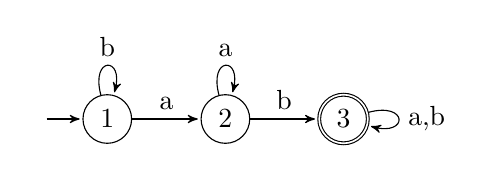
\begin{tikzpicture}[>=stealth',shorten >=1pt,auto,node distance=1.5cm,baseline=(current bounding box.center)]
        \tikzset{every state/.style={minimum size=0.2cm}}                    
        \node[initial,state]  (a1)      {1};
        \node[state] (b1)  [right of=a1]    {2};
        \node[state,accepting] [right of=b1](c1)      {3};
        \path[->]
            (a1)  edge  node {a} (b1)
            (a1)  edge[loop above]  node {b} (a1)
            (b1)  edge  node {b} (c1)
            (b1)  edge[loop above]  node {a} (b1)
            (c1)  edge[loop right]  node {a,b} (c1)
        ;
    \end{tikzpicture}
    \hspace{1.5cm}
    (b)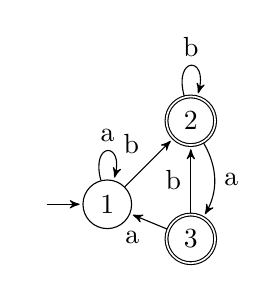
\begin{tikzpicture}[>=stealth',shorten >=1pt,auto,node distance=1.5cm,baseline=(current bounding box.center)]
        \tikzset{every state/.style={minimum size=0.2cm}}
        \node[initial,state]  (a1)      {1};
        \node[state,accepting] (b1)  [above right of=a1]    {2};
        \node[state,accepting] [below of=b1](c1)      {3};
        \path[->]
            (a1)  edge  node {b} (b1)
            (a1)  edge[loop above]  node {a} (a1)
            (b1)  edge[bend left]  node {a} (c1)
            (b1)  edge[loop above]  node {b} (b1)
            (c1)  edge  node {a} (a1)
            (c1)  edge  node {b} (b1)
        ;
    \end{tikzpicture}        

\end{problem}


\medskip\begin{problem}[Doplněk regulárního výrazu]
    
    Mějme následující regulární výraz nad abecedou $\Sigma=\{a,b\}$ a buď $L=L(R)$:
    \[
        R=((a + b)(a + b))^*ab
    \]
  
    \smallskip

    \begin{enumerate}[(a)]
        \item Sestrojte (co nejmenší) \emph{nedeterministický} konečný automat $A$ rozpoznávající $L$.
        \item Podmnožinovou konstrukcí převeďte $A$ na \emph{deterministický} konečný automat $B$.
        \item Z automatu $B$ sestrojte DFA $C$  rozpoznávající \emph{doplněk} jazyka $L$.
    \end{enumerate}

\end{problem}

\medskip

\section*{K procvičení a k zamyšlení}


\begin{problem}[Převod regulárního výrazu na automat]

    Zkonstruujte NFA rozpoznávající jazyky popsané následujícími regulárními výrazy:
    
    \vspace{-6pt}
    \begin{multicols}{2}
    
        \begin{enumerate}[(a)]\setlength\itemsep{0pt}
            \item $ab + ba$
            \item $((ab + c)+a(bc)^* + b)^*$
            \item $((ab + c)^*a(bc)^* + b)^*$
            \item $(01^* + 101)^*0^*1$
        \end{enumerate}
    
    \end{multicols}
    
\end{problem}


\begin{problem}[Převod automatu na regulární výraz]
    
    Sestrojte regulární výrazy pro jazyky rozpoznávané následujícími automaty.

    \vspace{-12pt}
    \begin{multicols}{2}
        \begin{enumerate}[(a)]
            \item 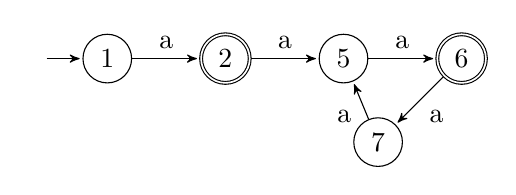
\begin{tikzpicture}[>=stealth',shorten >=1pt,auto,node distance=1.5cm,baseline=(current bounding box.north)]
                \tikzset{every state/.style={minimum size=0.2cm}}
                \node[initial,state]  (a1)      {1};
                \node[state,accepting] (b1)  [right of=a1]    {2};        
                \node[state] (c1)  [right of=b1]    {5};
                \node[state,accepting] (d1)  [right of=c1]    {6};
                \node[state] (e1)  [below left of=d1]    {7};
                \path[->]
                    (a1)  edge  node {a} (b1)
                    (b1)  edge  node {a} (c1)
                    (c1)  edge  node {a} (d1)
                    (d1)  edge  node {a} (e1)
                    (e1)  edge  node {a} (c1)
                ;
            \end{tikzpicture}

            \item 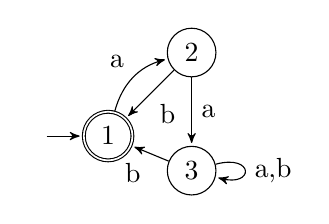
\begin{tikzpicture}[>=stealth',shorten >=1pt,auto,node distance=1.5cm,baseline=(current bounding box.north)]
                \tikzset{every state/.style={minimum size=0.2cm}}
                \node[initial,state,accepting]  (a1)      {1};
                \node[state] (b1)  [above right of=a1]    {2};
                \node[state] [below of=b1](c1)      {3};
                \path[->]
                    (a1)  edge [bend left] node {a} (b1)
                    (c1)  edge[loop right]  node {a,b} (c1)
                    (b1)  edge  node {a} (c1)
                    (b1)  edge  node {b} (a1)
                    (c1)  edge  node {b} (a1)
                ;
            \end{tikzpicture}

            \item 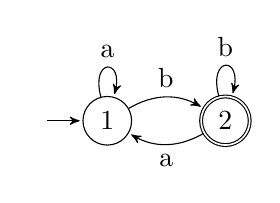
\begin{tikzpicture}[>=stealth',shorten >=1pt,auto,node distance=1.5cm,baseline=(current bounding box.north)]
                \tikzset{every state/.style={minimum size=0.2cm}}			
                \node[initial,state]  (a1)      {1};
                \node[state,accepting] (b1)  [right of=a1]    {2};
                \path[->]
                    (a1)  edge[bend left]  node {b} (b1)
                    (a1)  edge[loop above]  node {a} (a1)
                    (b1)  edge[bend left]  node {a} (a1)
                    (b1)  edge[loop above]  node {b} (b1)
                ;
            \end{tikzpicture}

            \item 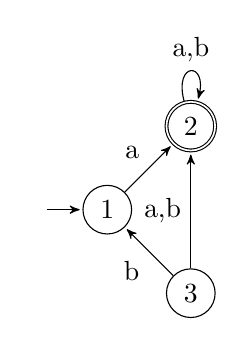
\begin{tikzpicture}[>=stealth',shorten >=1pt,auto,node distance=1.5cm,baseline=(current bounding box.north)]
                \tikzset{every state/.style={minimum size=0.2cm}}
                \node[initial,state]  (a1)      {1};
                \node[state,accepting] (b1)  [above right of=a1]    {2};
                \node[state] [below right of=a1](c1)      {3};
                \path[->]
                    (a1)  edge  node {a} (b1)
                    (b1)  edge[loop above]  node {a,b} (b1)
                    (c1)  edge  node {b} (a1)
                    (c1)  edge  node {a,b} (b1)
                ;
            \end{tikzpicture}
        \end{enumerate}
    \end{multicols}

\end{problem}

\vspace{-12pt}
\begin{problem}[Testování ekvivalence regulárních výrazů]
    Popište algoritmus na testování ekvivalence regulárních výrazů. Aplikujte ho na $(a + b)(a + b)^*$, $a(a + b)^* + b(a + b)^*$.
\end{problem}


\begin{problem}[Jsou regulární výrazy regulární?]

    Mějme konečnou abecedu $\Sigma$. Je jazyk sestávající ze všech regulárních výrazů nad abecedou $\Sigma$ regulárním jazykem?

\end{problem}


\section*{Bonus: Dvousměrné automaty}


\begin{problem}[Převod dvousměrného automatu]

    Uvažte následující dvousměrný DFA.

    \vspace{-6pt}
    \begin{multicols}{3}

        \begin{enumerate}[(a)]
            \item Určete jazyk rozpoznávaný tímto automatem.
            \item Určete funkce $f_w$, kongruenci $\sim$ pro $|w|\leq 4$.
            \item Převeďte ho na ekvivalentní jednosměrný konečný automat.
        \end{enumerate}

        \vspace{-8pt}
        \begin{center}
            \begin{tabular}{ r | c c }
                & a & b \\
                \hline
                $\to\ast p$ & $p,1$ & $q,-1$ \\
                $q$ & $r,1$ & \\
                $r$ & & $p,1$
            \end{tabular}
        \end{center}

        \begin{center}
            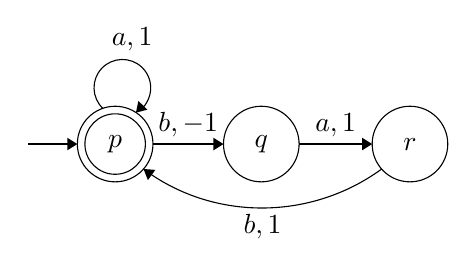
\begin{tikzpicture}[scale=0.16]
                \tikzstyle{every node}+=[inner sep=0pt]
                \draw [black] (10.1,-9.7) circle (3);
                \draw (10.1,-9.7) node {$p$};
                \draw [black] (10.1,-9.7) circle (2.4);
                \draw [black] (21.7,-9.7) circle (3);
                \draw (21.7,-9.7) node {$q$};
                \draw [black] (33.5,-9.7) circle (3);
                \draw (33.5,-9.7) node {$r$};
                \draw [black] (3.2,-9.7) -- (7.1,-9.7);
                \fill [black] (7.1,-9.7) -- (6.3,-9.2) -- (6.3,-10.2);
                \draw [black] (9.129,-6.874) arc (226.70189:-61.29811:2.25);
                \draw (11.45,-2.35) node [above] {$a,1$};
                \fill [black] (11.75,-7.21) -- (12.66,-6.97) -- (11.94,-6.28);
                \draw [black] (13.1,-9.7) -- (18.7,-9.7);
                \fill [black] (18.7,-9.7) -- (17.9,-9.2) -- (17.9,-10.2);
                \draw (15.9,-9.2) node [above] {$b,-1$};
                \draw [black] (24.7,-9.7) -- (30.5,-9.7);
                \fill [black] (30.5,-9.7) -- (29.7,-9.2) -- (29.7,-10.2);
                \draw (27.6,-9.2) node [above] {$a,1$};
                \draw [black] (31.254,-11.682) arc (-53.92224:-126.07776:16.054);
                \fill [black] (12.35,-11.68) -- (12.7,-12.56) -- (13.29,-11.75);
                \draw (21.8,-15.26) node [below] {$b,1$};
            \end{tikzpicture}
        \end{center}

    \end{multicols}

\end{problem}


\begin{problem}[Bez dvousměrných automatů to jde těžko]
    
    Pro daný DFA $A$ navrhněte NFA rozponávající jazyk $L'=\{\#w\#\ |\ ww^R\in L(A)\}$. (Bez použití dvousměrných automatů.)

\end{problem}


\begin{problem}[Konstrukce dvousměrného automatu]
    
    Buď $L$ regulární jazyk nad $\Sigma$ a $\#\notin\Sigma$. Sestrojte dvousměrný konečný automat rozpoznávající daný jazyk: 
    
    (a) $L' = \{\#w\#\mid ww^R \in L\}$\hfill (b) $L' = \{\#w\#\mid (\exists u \in\Sigma^*)\, wu \in L\ \& \ |w|=|u|\}$

\end{problem}


\end{document}
